\documentclass{beamer}
\mode<presentation>
\usepackage{amsmath,amssymb,mathtools}
\usepackage{textcomp}
\usepackage{gensymb}
\usepackage{adjustbox}
\usepackage{subcaption}
\usepackage{enumitem}
\usepackage{multicol}
\usepackage{listings}
\usepackage{url}
\usepackage{graphicx} % <-- needed for images
\def\UrlBreaks{\do\/\do-}

\usetheme{Boadilla}
\usecolortheme{lily}
\setbeamertemplate{footline}{
  \leavevmode%
  \hbox{%
  \begin{beamercolorbox}[wd=\paperwidth,ht=2ex,dp=1ex,right]{author in head/foot}%
    \insertframenumber{} / \inserttotalframenumber\hspace*{2ex}
  \end{beamercolorbox}}%
  \vskip0pt%
}
\setbeamertemplate{navigation symbols}{}

\lstset{
  frame=single,
  breaklines=true,
  columns=fullflexible,
  basicstyle=\ttfamily\tiny   % tiny font so code fits
}

\numberwithin{equation}{section}

% ---- your macros ----
\providecommand{\nCr}[2]{\,^{#1}C_{#2}}
\providecommand{\nPr}[2]{\,^{#1}P_{#2}}
\providecommand{\mbf}{\mathbf}
\providecommand{\pr}[1]{\ensuremath{\Pr\left(#1\right)}}
\providecommand{\qfunc}[1]{\ensuremath{Q\left(#1\right)}}
\providecommand{\sbrak}[1]{\ensuremath{{}\left[#1\right]}}
\providecommand{\lsbrak}[1]{\ensuremath{{}\left[#1\right.}}
\providecommand{\rsbrak}[1]{\ensuremath{\left.#1\right]}}
\providecommand{\brak}[1]{\ensuremath{\left(#1\right)}}
\providecommand{\lbrak}[1]{\ensuremath{\left(#1\right.}}
\providecommand{\rbrak}[1]{\ensuremath{\left.#1\right)}}
\providecommand{\cbrak}[1]{\ensuremath{\left\{#1\right\}}}
\providecommand{\lcbrak}[1]{\ensuremath{\left\{#1\right.}}
\providecommand{\rcbrak}[1]{\ensuremath{\left.#1\right\}}}
\theoremstyle{remark}
\newtheorem{rem}{Remark}
\newcommand{\sgn}{\mathop{\mathrm{sgn}}}
\providecommand{\abs}[1]{\left\vert#1\right\vert}
\providecommand{\res}[1]{\Res\displaylimits_{#1}}
\providecommand{\norm}[1]{\lVert#1\rVert}
\providecommand{\mtx}[1]{\mathbf{#1}}
\providecommand{\mean}[1]{E\left[ #1 \right]}
\providecommand{\fourier}{\overset{\mathcal{F}}{ \rightleftharpoons}}
\providecommand{\system}{\overset{\mathcal{H}}{ \longleftrightarrow}}
\providecommand{\dec}[2]{\ensuremath{\overset{#1}{\underset{#2}{\gtrless}}}}
\newcommand{\myvec}[1]{\ensuremath{\begin{pmatrix}#1\end{pmatrix}}}
\newcommand{\mydet}[1]{\ensuremath{\begin{vmatrix}#1\end{vmatrix}}}

\newenvironment{amatrix}[1]{%
  \left(\begin{array}{@{}*{#1}{c}|c@{}}
}{%
  \end{array}\right)
}

\newcommand{\myaugvec}[2]{\ensuremath{\begin{amatrix}{#1}#2\end{amatrix}}}
\let\vec\mathbf
% ---------------------


\title{5.2.59}
\author{Rushil Shanmukha Srinivas \\EE25BTECH11057 \\ Electrical Enggineering ,\\IIT Hyderabad.}

\date{\today} 
\begin{document} 

\begin{frame}
\titlepage
\end{frame}

\section*{Outline}
\begin{frame}
\tableofcontents
\end{frame}
\section{Problem}
\begin{frame}
\frametitle{Problem Statement}
\textbf{Question} : Solve the system of equations

\begin{align}
2x +3y + 3z &= 5\\
x -2y +z &= -4\\
3x -y -2z &= 3
\end{align}

\end{frame}
\section{Solution}
\subsection{Augmented Matrix and Gaussian Elimination}
\begin{frame}
\frametitle{Augmented Matrix and Gaussian Elimination}
%\framesubtitle{Literature}
\textbf{Solution:}


The system of equations in matrix form is :

\begin{align}
  \myvec{2 & 3 & 3\\1 & -2 & 1\\3 & -1 & -2}\myvec{x\\y\\z} &= \myvec{5\\-4\\3}
\end{align}

Forming the augmented matrix,

\begin{align}
  \myaugvec{3}{2 & 3 & 3 & 5\\ 1 & -2 & 1 & -4\\3 & -1 & -2 & 3}
\end{align}

Using Gaussian elimination,

\begin{align}
  \myaugvec{3}{2 & 3 & 3 & 5\\ 1 & -2 & 1 & -4\\3 & -1 & -2 & 3}
  \xleftrightarrow[\;R_2 \to 2R_2 -R_1\;]{\;R_3 \to 2R_3 - 3R_1}
  \myaugvec{3}{2 & 3 & 3 & 5\\0 & -7 & -1 & -13\\0 & -11 & -13 & -9}
  \end{align}
  \end{frame}
  \begin{frame}
  \begin{align}
   \myaugvec{3}{2 & 3 & 3 & 5\\0 & -7 & -1 & -13\\0 & -11 & -13 & -9}
  \xleftrightarrow{R_3 \to R_3 -\tfrac{11}{7}R_2}
  \myaugvec{3}{2 & 3 & 3 & 5\\0 & -7 & -1 & -13\\0 & 0 & \tfrac{-80}{7} & \tfrac{80}{7}}
\end{align}

Using back substitution we get :

\begin{align}
  \tfrac{-80}{7} z &= \tfrac{80}{7}\\ 
  z &= -1\\
  -7y - z &= -13\\
  -7y +1 &= -13\\
  7y &= 14\\
  y &= 2\\
  2x + 3y + 3z &= 5\\
  2x + 3 &= 5\\
  x &= 1
\end{align}

\end{frame}
\begin{frame}
 \frametitle{Solution for System of Equations}
Therefore the solution for the system of equations is : 

\begin{align}
  \myvec{1\\2\\-1}
\end{align}


\end{frame}
\subsection{Plots}
\begin{frame}
\frametitle{Plots}
\begin{figure}
\centering
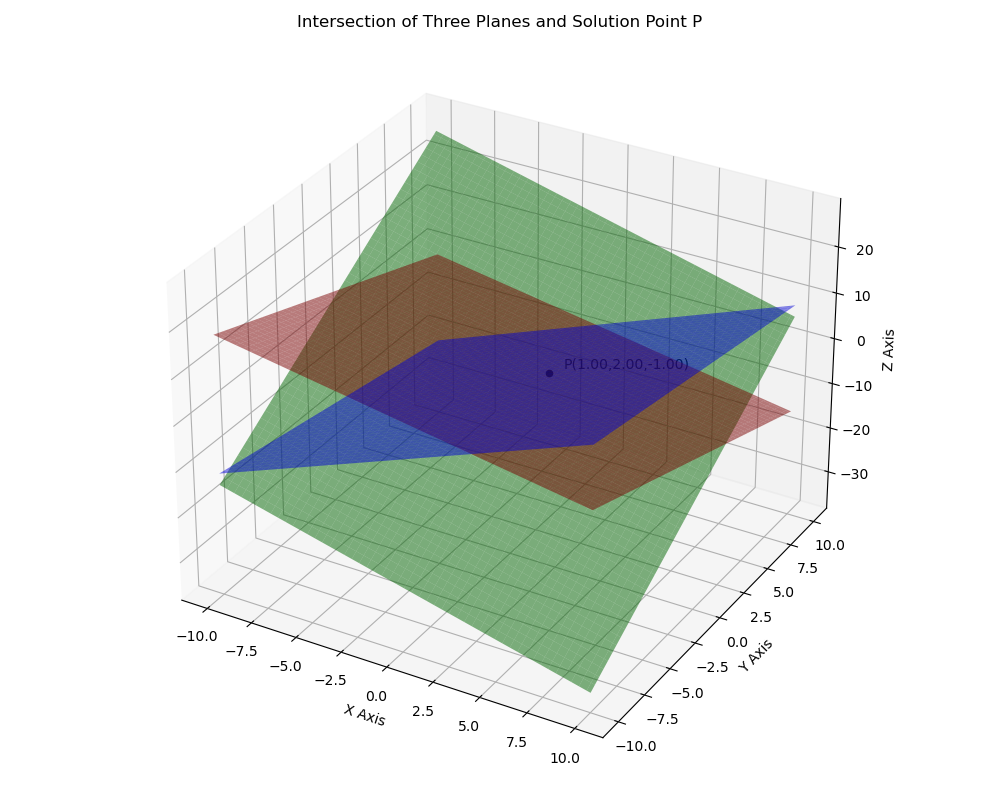
\includegraphics[width=0.9\columnwidth]{figs/solution.png}
\caption{fig : Representation of Planes}
\label{Fig8}
\end{figure}
\end{frame}
\section{C Code}
\begin{frame}[fragile]
\frametitle{C Code }
\begin{lstlisting}[language=C]  
#include <stdio.h>

// Function to compute determinant of a 3x3 matrix
double det3(double m[3][3]) {
    return m[0][0]*(m[1][1]*m[2][2] - m[1][2]*m[2][1])
         - m[0][1]*(m[1][0]*m[2][2] - m[1][2]*m[2][0])
         + m[0][2]*(m[1][0]*m[2][1] - m[1][1]*m[2][0]);
}

// Function to solve the system using Cramer's rule
// solution[0] -> x, solution[1] -> y, solution[2] -> z
void solve_system(double *solution) {
    double a[3][3] = {
        {2, 3, 3},
        {1, -2, 1},
        {3, -1, -2}
    };
    double b[3] = {5, -4, 3};

    double m[3][3];

    // Determinant of coefficient matrix
    double detA = det3(a);

    if(detA == 0) {
        solution[0] = solution[1] = solution[2] = 0.0;
        return;
    }

    // Dx (replace 1st column with b)
    for(int i=0;i<3;i++) for(int j=0;j<3;j++) m[i][j]=a[i][j];
    for(int i=0;i<3;i++) m[i][0] = b[i];
    double detX = det3(m);
    \end{lstlisting}
    \end{frame}
    \begin{frame}[fragile]
    \begin{lstlisting}

    // Dy (replace 2nd column with b)
    for(int i=0;i<3;i++) for(int j=0;j<3;j++) m[i][j]=a[i][j];
    for(int i=0;i<3;i++) m[i][1] = b[i];
    double detY = det3(m);

    // Dz (replace 3rd column with b)
    for(int i=0;i<3;i++) for(int j=0;j<3;j++) m[i][j]=a[i][j];
    for(int i=0;i<3;i++) m[i][2] = b[i];
    double detZ = det3(m);

    solution[0] = detX / detA;
    solution[1] = detY / detA;
    solution[2] = detZ / detA;
}

// Optional main function (for direct C execution)
// This will be ignored when creating shared object
int main() {
    double solution[3];
    solve_system(solution);

    printf("Solution:\n");
    printf("x = %lf\n", solution[0]);
    printf("y = %lf\n", solution[1]);
    printf("z = %lf\n", solution[2]);

    return 0;
}

\end{lstlisting}
\end{frame}

\section{Python Code}
\begin{frame}[fragile]
\frametitle{Python : call\_c.py}
\begin{lstlisting}
import ctypes

# Load the shared object file
solver = ctypes.CDLL('./solve.so')

# Tell Python about the function signature
solver.solve_system.argtypes = [ctypes.POINTER(ctypes.c_double)]
solver.solve_system.restype = None

# Create an array of 3 doubles to hold the solution
solution = (ctypes.c_double * 3)()

# Call the C function
solver.solve_system(solution)

# Print the results
print("Solution from C shared object:")
print(f"x = {solution[0]}")
print(f"y = {solution[1]}")
print(f"z = {solution[2]}")

\end{lstlisting}
\end{frame}

\begin{frame}[fragile]
\frametitle{Python Code for Plotting}
\begin{lstlisting}[language=Python]


import os
import numpy as np
import matplotlib.pyplot as plt

# for saving figure in figs folder
figs_folder = os.path.join("..", "figs")

# Define system of equations
# 2*x +3*y +3*z = 5
# 1*x -2*y +1*z = -4
# 3*x -1*y -2*z = 3

A = np.array([[2, 3, 3],
              [1, -2, 1],
              [3, -1, -2]], dtype=float)

b = np.array([5, -4, 3], dtype=float)

# Solve using numpy
solution = np.linalg.solve(A, b)
x, y, z = solution
print("Solution from NumPy:", solution)

# Create meshgrid for plotting planes
x_vals = np.linspace(-10, 10, 100)
y_vals = np.linspace(-10, 10, 100)
X, Y = np.meshgrid(x_vals, y_vals)

# Plane 1: 2x + 3y + 3z = 5 -> z = (5 - 2x - 3y)/3
Z1 = (5 - 2*X - 3*Y)/3
\end{lstlisting}
\end{frame}
\begin{frame}[fragile]
\begin{lstlisting}

# Plane 2: x - 2y + z = -4 -> z = (-4 -x + 2y)
Z2 =(-4 -X +2*Y)

# Plane 3: 3x - y - 2z = 3 -> z = (-3 + 3x - y )/2
Z3 = (-3 + 3*X - Y)/2

# Plotting
fig = plt.figure(figsize=(10, 8))
ax = fig.add_subplot(111, projection="3d")

# Plot the planes
ax.plot_surface(X, Y, Z1, alpha=0.5, color="red")
ax.plot_surface(X, Y, Z2, alpha=0.5, color="green")
ax.plot_surface(X, Y, Z3, alpha=0.5, color="blue")

# Plot the solution point
ax.scatter(x, y, z, color="black")
ax.text(x+0.5, y+0.5, z+0.5,
        f"P({x:.2f},{y:.2f},{z:.2f})",
        fontsize=10, color="black")

# Axes labels and title
ax.set_xlabel("X Axis")
ax.set_ylabel("Y Axis")
ax.set_zlabel("Z Axis")
ax.set_title("Intersection of Three Planes and Solution Point P")
ax.grid(True)

# Save figure
plt.tight_layout()
fig.savefig(os.path.join(figs_folder, "solution.png"))
plt.show()


\end{lstlisting}
\end{frame}

\end{document}
  